\subsection{Impostazioni generali}

\par Il sistema, nella sezione in alto a destra, presenta due simboli: una rotella e un omino stilizzato. La rotella dà accesso alle impostazioni descritte di seguito, mentre l'omino stilizzato permette l'accesso al sistema come admin (\sezione{sec:autenticazione}).

\begin{figure}[H]
  \centering
  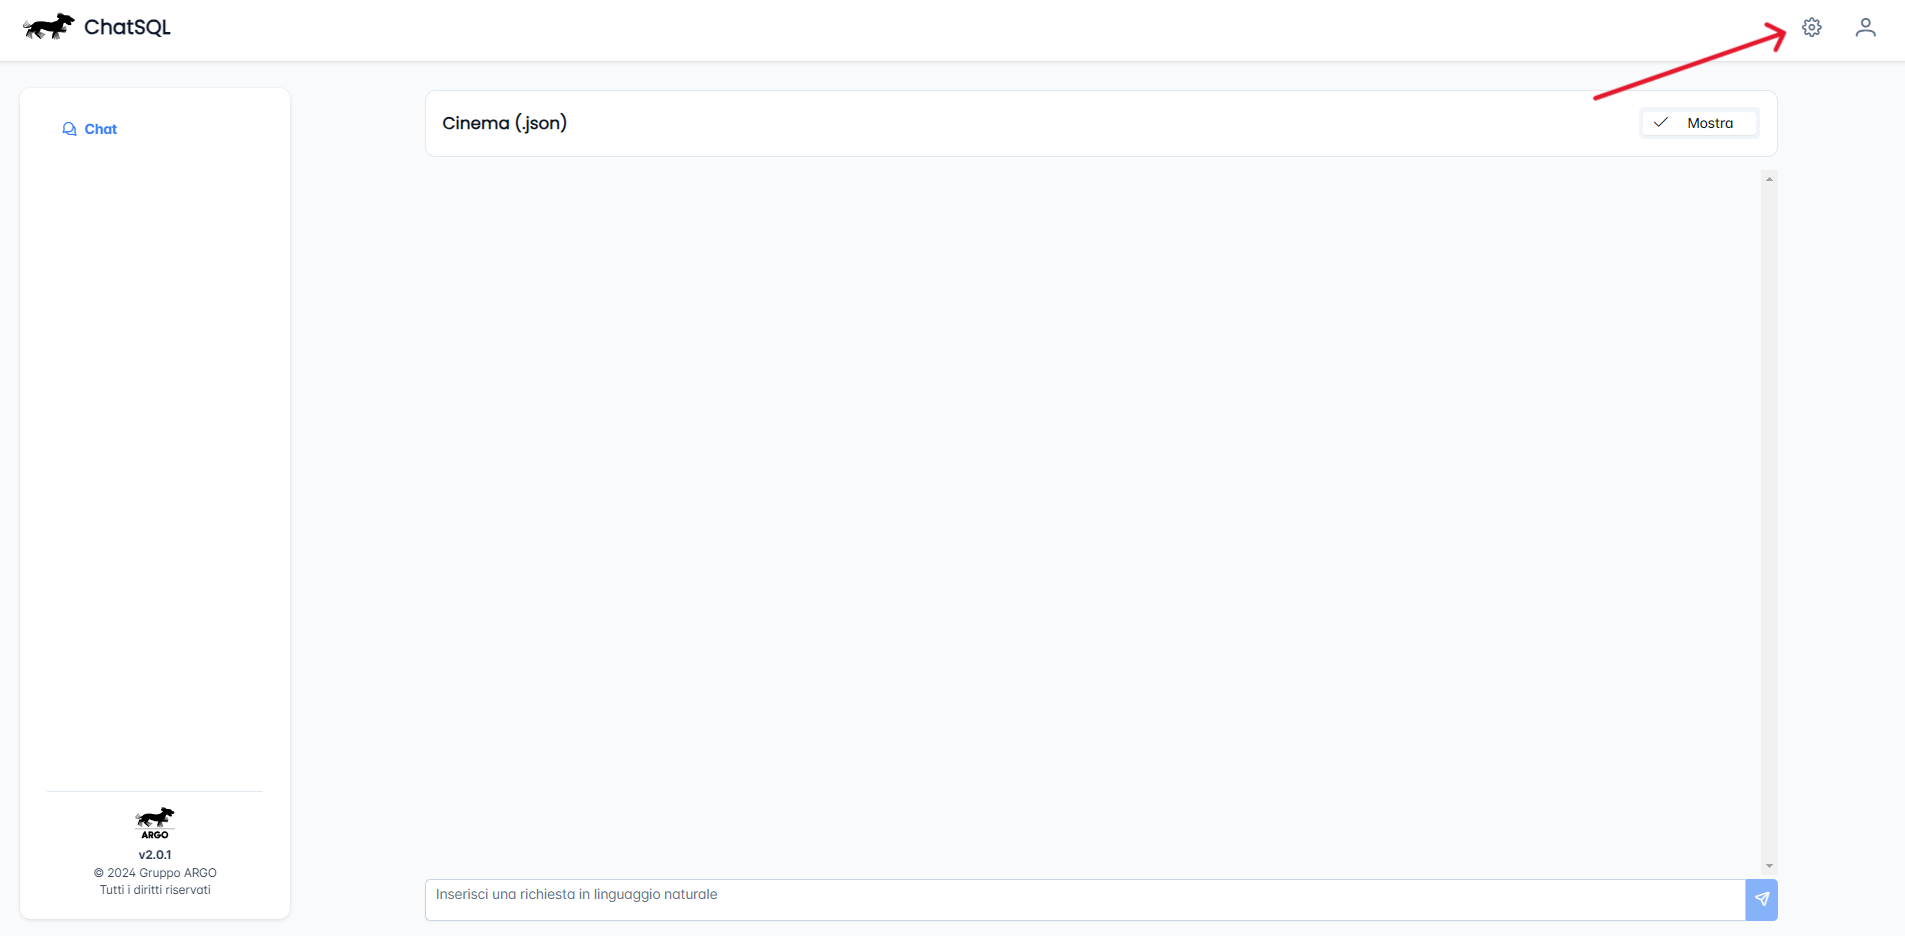
\includegraphics[width=\textwidth]{assets/chat_generale.png}
  \caption{Icona impostazioni}
\end{figure}

\par Dopo aver cliccato sull'icona delle impostazioni 
\includegraphics[height=1.2em]{assets/settings_icon.png}, si aprirà un menu con le seguenti opzioni:
\begin{enumerate}
    \item Dimensione del testo;
    \item Modalità di visualizzazione (chiara o scura);
    \item Lingua del sistema.
\end{enumerate}

\begin{figure}[H]
  \centering
  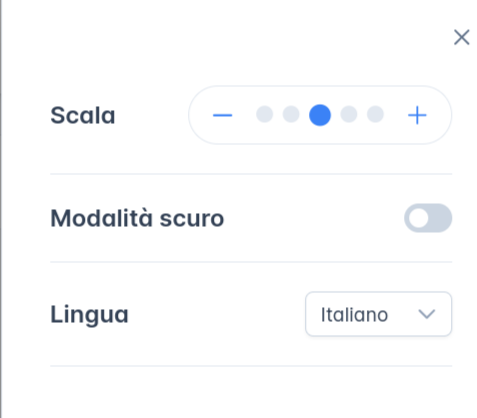
\includegraphics[width=0.50\textwidth]{assets/menu_config.png}
  \caption{Menu laterale delle impostazioni di sistema}
\end{figure}

\subsubsection{Scala di grandezza del testo}

\par Il sistema permette all'Utente di impostare la grandezza dei caratteri del testo tramite una scala di 5 misure diverse. Per modificare la dimensione, è necessario cliccare i pulsanti ``-'' o ``+'' presenti affianco alla voce ``Scala''. Questi pulsanti consentono rispettivamente di rimpicciolire o ingrandire il testo. L'Utente può quindi adattare la dimensione dell'interfaccia alle proprie esigenze, migliorando così l'accessibilità, la personalizzazione e il comfort visivo.

\begin{figure}[H]
  \centering
  %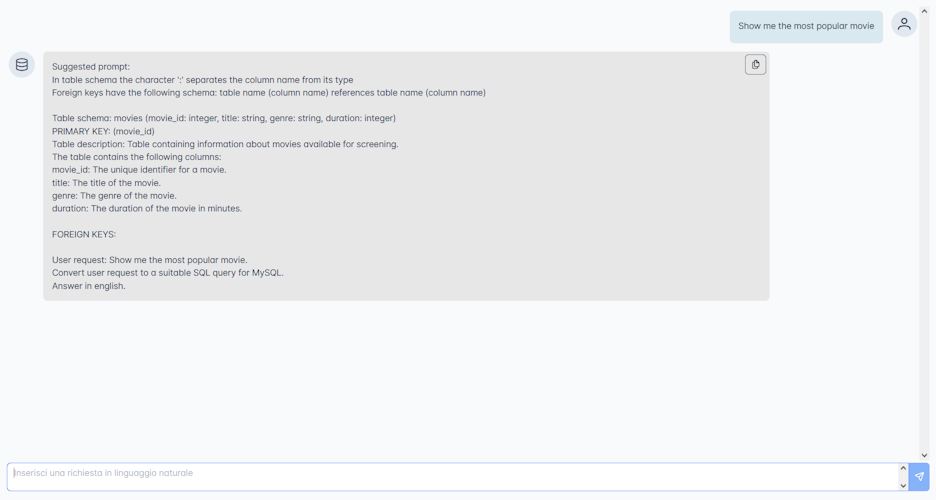
\includegraphics[width=\textwidth]{assets/chat_example.png}
  \caption{Immagine con freccia nella scala}
\end{figure}

\subsubsection{Tema chiaro o scuro} \label{sec:tema}

\par Il sistema consente di impostare la modalità di visualizzazione dell'interfaccia. Di default, la modalità è chiara, con lo sfondo del sistema di colore bianco. Tuttavia, è possibile attivare il tema scuro, con sfondo nero, cliccando sul pulsante accanto alla voce ``Modalità scuro''.

\begin{figure}[H]
  \centering
  %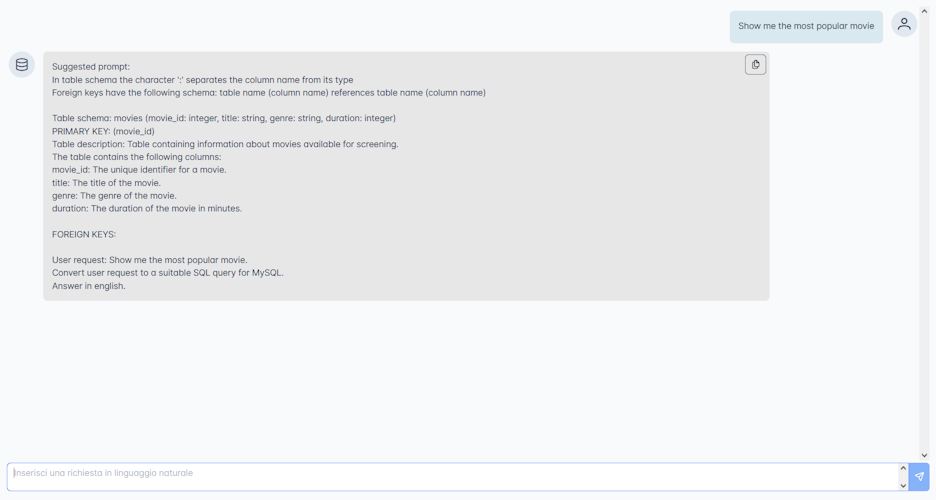
\includegraphics[width=\textwidth]{assets/chat_example.png}
  \caption{Immagine con freccia nella modalità notturna}
\end{figure}

\subsubsection{Lingua del sistema} \label{sec:lingua}

\par Il sistema consente di impostare la lingua dell'applicazione, applicandola a tutti gli elementi dell'interfaccia grafica, come i testi dei pulsanti o le voci di menu. Tuttavia, la lingua selezionata per l'interfaccia non influisce sul contenuto del \glossario{prompt} o del \glossario{debug} (si veda la \sezione{sec:lingua-chat} per maggiori dettagli). L'Utente può scegliere tra le seguenti lingue:
\begin{itemize}
  \item Inglese;
  \item Italiano (lingua predefinita).
\end{itemize}

\begin{figure}[H]
  \centering
  %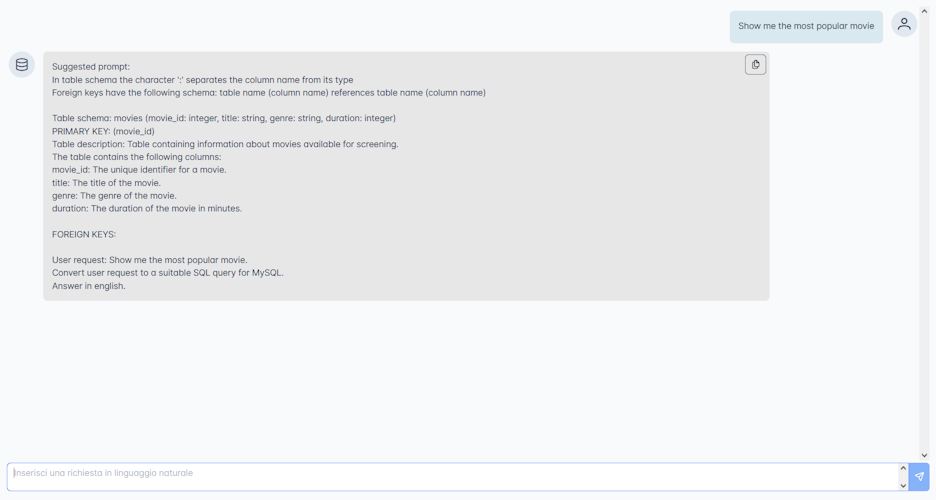
\includegraphics[width=\textwidth]{assets/chat_example.png}
  \caption{Immagine con freccia nella lingua}
\end{figure}

\par Le modifiche apportate vengono memorizzate automaticamente, e applicate alla successiva apertura dell'applicazione. Per chiudere la barra laterale delle impostazioni, è necessario cliccare sulla ``x'' in alto a destra, dopodiché si tornerà al sistema con le impostazioni selezionate.
